\documentclass{article}
\begin{document}
Intro text with $x$ and \verb|$not math$| here.
\begin{align}
  a &= b + c \label{l1}\\
  d &= e \nonumber \\
    &= f \label{l2}\\[2pt]
  g &= \begin{cases} 1 & x>0 \\ 0 & x \le 0 \end{cases}
\end{align}
\begin{align*}
  p &= q \\
  &= r
\end{align*}
\begin{gather}
  u = 1 \\
  v = 2
\end{gather}
\begin{multline}
  m_1 + m_2 + m_3 \\
  + m_4 = 0
\end{multline}
\begin{equation}
  \begin{split} s &= t \\ &= w \end{split}
\end{equation}
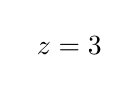
\begin{tikzpicture}
\node {$z = 3$};
\end{tikzpicture}
\begin{verbatim}
$verbatim = 1$
\end{verbatim}
\begin{figure}
\caption{Caption text with $k=1$ lives in a float}
\end{figure}
\begin{equation}\label{x}
\xi = \ref{eq:one}
\end{equation}
\end{document}
